\documentclass[11pt]{article}

\usepackage[utf8]{inputenc}
\usepackage[T1]{fontenc}
\usepackage{lmodern}
\usepackage{amsmath, amssymb, mathtools}
\usepackage{bm}
\usepackage{graphicx}
\usepackage{xcolor}
\usepackage{hyperref}
\usepackage[capitalize,noabbrev]{cleveref}
\usepackage{geometry}
\usepackage{caption}
\usepackage{subcaption}
\usepackage[numbers]{natbib}
\geometry{a4paper, margin=2.4cm}

\newcommand{\bxi}{\boldsymbol{\xi}}
\newcommand{\bx}{\bm{x}}
\newcommand{\avg}[1]{\langle #1 \rangle}
\newcommand{\e}{{\mathrm{e}}}
\newcommand{\dd}{{\mathrm{d}}}
\newcommand{\Bnet}{\beta_{\mathrm{net}}}
\newcommand{\phieq}{\phi_{\mathrm{eq}}}
\newcommand{\fret}{f_{\mathrm{ret}}}
\newcommand{\acGauss}{\alpha_c^{\mathrm{G}}}
\newcommand{\acBd}{\alpha_c^{\mathrm{bd}}}
\newcommand{\acSd}{\alpha_c^{\mathrm{sd}}}
\newcommand{\acSp}{\alpha_c^{\mathrm{sp}}}
\newcommand{\Tsp}{T_{\mathrm{sp}}}

\title{\bfseries Saddle-Dominated Capacity of LSE Dense Associative Memory:\\
status report}
\author{}
\date{}

\begin{document}
\maketitle

% =========================================================================
\begin{abstract}
\noindent
The log-sum-exp (LSE) Dense Associative
Memory~\citep{ramsauer2021hopfield} stores $M$ unit vectors
$\bxi^\mu$ ($\mu = 1, \dots, M$) on the $N$-sphere of radius
$\sqrt{N}$ and assigns to each chain state $\bx$ the energy
$H(\bx) = -\Bnet^{-1} \ln \sum_\mu \exp(\Bnet\,\bx \cdot \bxi^\mu)$,
with $\Bnet$ the kernel sharpness (inverse variance).  At load
$\alpha = \ln M / N$ and external temperature $T$, the question is
whether a chain at $\bxi^1$ stays close to it.

Ramsauer et al.\ proved $\alpha_c = 1/2$ at $T = 0$ by modelling the
inter-pattern overlaps
$\varphi_{1\mu} = \bxi^1 \cdot \bxi^\mu / N$ as Gaussian.  A
thermodynamic companion~\citep{icml2026theory} recast this as a
crossover between the retrieval free energy $\fret(T)$ and a
noise-floor energy $u_{\mathrm{noise}}(\alpha)$, with the same
$T \to 0$ value under the Gaussian.  A second
companion~\citep{petrova2026metastable} replaced the Gaussian by the
exact density of $\varphi_{1\mu}$ on the sphere; for the LSR kernel
this raised the threshold from $0.25$ to $\approx 0.347$.

This report applies the exact-density correction to LSE.  The
spurious partition sum $S_{\mathrm{spur}} = \sum_{\mu \neq 1}
\exp(\Bnet N \varphi_{1\mu})$ acquires an interior saddle at
$\varphi^* = (\sqrt 5 - 1)/2$ with value
$g_{\max} = \tfrac12 \ln \varphi^* + \varphi^* \approx 0.3774$.  From
$u_{\mathrm{noise}}(\alpha) = 1 - (\alpha + g_{\max})/\Bnet$ and the
crossover condition $\fret(T) = u_{\mathrm{noise}}$, the boundary at
$\Bnet = 1$ is $\acSd(T) = 1 - g_{\max} - \fret(T)$, so
$\acSd(0) \approx 0.6226$, not $0.5$.  Transplanting the LSR
support-edge derivation to LSE gives a different formula
$\acBd(T)$ that diverges at $T \to 0$; it is correct only for
$\alpha < 0.241$ (where the saddle leaves the support).

The single-pattern spinodal $\Tsp(\alpha)$, the temperature at which
the retrieval basin loses local stability, lies above $\acSd$ at
$T > 0$ and meets it at the same endpoint $(1 - g_{\max},\,0)$.  In
leading order $\acSp(T) = \phieq(T) - g_{\max}$, where
$\phieq(T) = \tfrac12(-T + \sqrt{T^2 + 4})$ is the basin minimum
overlap.

Numerical status: a Monte Carlo heatmap at $N = 25$ over
$\alpha \in [0.20, 0.70]$, $T \in [0.025, 0.500]$ from two MC variants
(direct, semismart) and a cold-init spinodal probe at $N \in
\{50, 100, 1000\}$ for $\alpha \in [0.20, 0.60]$.  $\acSd$ tracks the
$N = 25$ residual at $\alpha \gtrsim 0.45$.  The empirical spinodal
anchors sit below $\acSp$ across most of the range, except at
$(\alpha, N) = (0.60, 1000)$ where the deviation is an NLO correction
to the spinodal itself (verified by a Kramers budget calculation).
A list of remaining tasks closes the report.
\end{abstract}

% =========================================================================
\section{What we want}
\label{sec:want}

\paragraph{Model.}
A Dense Associative Memory~\citep{krotov2016dense} stores patterns
$\bxi^\mu \in \mathbb{R}^N$, $\mu = 1, \dots, M$, by encoding them as
minima of an energy function $H : \mathbb{R}^N \to \mathbb{R}$.
Retrieval of $\bxi^1$ from a noisy cue is the Metropolis dynamics of
$\bx$ under $H$ at external temperature $T$.  Both patterns and
chain lie on the $N$-sphere of radius $\sqrt N$:
$|\bxi^\mu|^2 = |\bx|^2 = N$.

The log-sum-exp (LSE) kernel~\citep{ramsauer2021hopfield} defines
\begin{equation}
H_{\mathrm{LSE}}(\bx) = -\frac{1}{\Bnet}\,
   \ln\!\sum_{\mu=1}^{M} \exp(\Bnet\,\bx \cdot \bxi^\mu),
\label{eq:lse}
\end{equation}
where $\Bnet$ is the kernel sharpness (inverse variance) and has no
relation to the external temperature.  Throughout this report
$\Bnet = 1$.

\paragraph{Overlaps and load.}
The chain--target and inter-pattern overlaps are
\begin{equation}
\varphi_1(\bx) = \frac{\bxi^1 \cdot \bx}{N},
\qquad
\varphi_{1\mu} = \frac{\bxi^1 \cdot \bxi^\mu}{N},
\label{eq:overlaps}
\end{equation}
both in $[-1, 1]$.  Perfect retrieval is $\varphi_1 = 1$.  The pattern
count scales as
\begin{equation}
M = \e^{\alpha N},
\qquad \alpha = \frac{\ln M}{N},
\label{eq:alpha}
\end{equation}
and $\alpha$ is the load.  For uniformly distributed patterns on
the sphere, $\varphi_{1\mu}$ has the exact density
\begin{equation}
f(\varphi) = \frac{(1 - \varphi^2)^{(N-3)/2}}
                  {B((N-1)/2,\,1/2)},
\qquad \varphi \in [-1, 1],
\label{eq:exact-density}
\end{equation}
with mean $0$ and variance $1/N$.

\paragraph{Question.}
At $T = 0$, Ramsauer et al.\ proved that retrieval succeeds up to
$\alpha_c = 1/2$, replacing $f(\varphi)$ by the Gaussian
$\mathcal{N}(0, 1/N)$.  The thermodynamic recast of the same
argument~\citep{icml2026theory} produces a smooth boundary
$\alpha_c(T)$ at finite $T$, equal to $1/2$ at $T = 0$ under the
same Gaussian.  The companion LSR paper~\citep{petrova2026metastable}
showed that using \eqref{eq:exact-density} instead of the Gaussian
shifts the LSR threshold from $0.25$ to $\approx 0.347$.  This
report asks: what does the exact-density correction give for LSE?

% =========================================================================
\section{Free energy framework}
\label{sec:framework}

The boundary $\alpha_c(T)$ comes from a competition between two
energies per spin: the retrieval free energy $\fret(T)$ and the
noise-floor energy $u_{\mathrm{noise}}(\alpha)$.  We derive both
explicitly.

\paragraph{Retrieval free energy $\fret(T)$.}
For a chain in the basin of $\bxi^1$ ($\varphi_1 \approx 1$,
$\varphi_{1\mu} \approx 0$ for $\mu \neq 1$), the sum in
\eqref{eq:lse} is dominated by $\mu = 1$:
\begin{equation}
\frac{H_{\mathrm{LSE}}(\bx)}{N}
   \;\approx\; -\frac{1}{\Bnet N}\,\ln \exp(\Bnet N \varphi_1)
   \;=\; -\varphi_1.
\label{eq:Hret}
\end{equation}
We define the energy per spin relative to the retrieval baseline,
\begin{equation}
u(\varphi_1) \;=\; 1 + \frac{H_{\mathrm{LSE}}}{N} \;=\; 1 - \varphi_1,
\label{eq:u}
\end{equation}
so $u(1) = 0$ at perfect retrieval and $u(0) = 1$ at zero overlap.
The geometric entropy of the $(N-1)$-sphere at fixed
$\varphi_1 = \phi$ is, per spin,
\begin{equation}
s(\phi) \;=\; \tfrac12 \ln(1 - \phi^2),
\label{eq:s}
\end{equation}
negative on $(0, 1)$~\citep{icml2026theory}.  The retrieval free
energy at overlap $\phi$ is
\begin{equation}
f(\phi, T) = u(\phi) - T\,s(\phi)
          = (1 - \phi) - \tfrac{T}{2}\,\ln(1 - \phi^2).
\label{eq:f-phi}
\end{equation}
Minimising in $\phi$, $\partial f/\partial \phi = 0$ gives
$T \phi = 1 - \phi^2$ and the basin overlap
\begin{equation}
\phieq(T) \;=\; \tfrac12 \bigl(-T + \sqrt{T^2 + 4}\bigr),
\qquad \phieq(0) = 1.
\label{eq:phieq}
\end{equation}
The retrieval free energy is the value at the minimum:
\begin{equation}
\fret(T) \;=\; f(\phieq(T), T)
   \;=\; (1 - \phieq) - \tfrac{T}{2}\,\ln(1 - \phieq^2).
\label{eq:fret}
\end{equation}

\paragraph{Noise-floor energy $u_{\mathrm{noise}}(\alpha)$.}
A chain uncorrelated with $\bxi^1$ has $\varphi_1 \approx 0$, so the
$\mu = 1$ term in \eqref{eq:lse} is comparable to the others and the
sum is dominated by the spurious patterns
\begin{equation}
S_{\mathrm{spur}}
   \;=\; \sum_{\mu \neq 1} \exp(\Bnet N \varphi_{1\mu}).
\label{eq:Sspur}
\end{equation}
For such a chain
$H_{\mathrm{LSE}}/N \approx -(\Bnet N)^{-1}\,\ln S_{\mathrm{spur}}$,
and by the convention \eqref{eq:u},
\begin{equation}
u_{\mathrm{noise}} \;=\; 1 - \frac{1}{\Bnet N}\,\ln S_{\mathrm{spur}}.
\label{eq:unoise-def}
\end{equation}
Replacing the discrete sum by an integral over the density
\eqref{eq:exact-density}, with $M = \e^{\alpha N}$,
\begin{equation}
S_{\mathrm{spur}}
   \;\approx\;
   M \int_{-1}^{1} f(\varphi)\,\exp(\Bnet N \varphi)\,\dd\varphi
   \;=\; \e^{\alpha N}
        \int_{-1}^{1} \e^{N\,g(\varphi)}\,\dd\varphi,
\label{eq:Sspur-integral}
\end{equation}
where we have set the integrand exponent (per spin) to
\begin{equation}
g(\varphi) \;\equiv\;
   \tfrac12 \ln(1 - \varphi^2) + \Bnet\,\varphi,
\label{eq:g}
\end{equation}
using $f(\varphi) \propto \exp[(N/2)\ln(1-\varphi^2)]$ at large $N$.
Evaluating \eqref{eq:Sspur-integral} by saddle in the large-$N$ limit,
\begin{equation}
\frac{1}{N}\,\ln S_{\mathrm{spur}}
   \;\approx\; \alpha + g_{\max},
\qquad
g_{\max} \;\equiv\; \max_{\varphi}\, g(\varphi).
\label{eq:lnSspur}
\end{equation}
Substituting into \eqref{eq:unoise-def}:
\begin{equation}
\boxed{\;
u_{\mathrm{noise}}(\alpha)
   \;=\; 1 - \frac{\alpha + g_{\max}}{\Bnet}.
\;}
\label{eq:unoise}
\end{equation}

\paragraph{Crossover.}
The two energies cross at $\alpha_c(T)$:
\begin{equation}
\fret(T) \;=\; u_{\mathrm{noise}}(\alpha_c)
\;\;\Longrightarrow\;\;
\alpha_c(T) \;=\; \Bnet\,\bigl[1 - \fret(T)\bigr] - g_{\max}.
\label{eq:master}
\end{equation}
For $\Bnet = 1$:
\begin{equation}
\boxed{\;
\alpha_c(T) \;=\; 1 - g_{\max} - \fret(T).
\;}
\label{eq:master-1}
\end{equation}
The three predictions of \Cref{sec:formulas} differ only in the value
of $g_{\max}$, determined by which $f(\varphi)$ and which integration
range one substitutes into \eqref{eq:Sspur-integral}.

% =========================================================================
\section{Three boundary formulas}
\label{sec:formulas}

Three choices of density and integration range, three values of
$g_{\max}$, three boundaries.

\paragraph{Gaussian density.}
Replace $f(\varphi)$ by the moment-matched Gaussian
$\sqrt{N/2\pi}\,\exp(-N \varphi^2 / 2)$.  The integrand exponent
becomes $g_G(\varphi) = -\tfrac12 \varphi^2 + \Bnet \varphi$, monotone
increasing on $[-1, 1]$ for $\Bnet = 1$.  The integral is dominated by
the upper cutoff, set by the typical maximum of $M$ Gaussian samples:
$M \cdot \Pr_G(\varphi_{1\mu} > \varphi_{\max}^{(G)}) = 1$ gives
$\varphi_{\max}^{(G)}(\alpha) = \sqrt{2\alpha}$.  At this edge,
$g_G(\varphi_{\max}^{(G)}) = \sqrt{2\alpha} - \alpha$, so by
\eqref{eq:lnSspur} and \eqref{eq:unoise}
$u_{\mathrm{noise}}^{(G)} = 1 - \sqrt{2\alpha}$.  The crossover
\eqref{eq:master-1} reads $1 - \sqrt{2 \acGauss} = \fret(T)$, hence
\begin{equation}
\acGauss(T) = \tfrac12 \bigl[1 - \fret(T)\bigr]^2,
\qquad \acGauss(0) = \tfrac12.
\label{eq:acgauss}
\end{equation}

\paragraph{Exact density, support edge.}
Keep the exact density \eqref{eq:exact-density} but restrict the
integration to the support edge $\varphi_{\max}(\alpha)$, defined by
$M \cdot \Pr_f(\varphi_{1\mu} > \varphi_{\max}) = 1$:
\begin{equation}
\varphi_{\max}(\alpha) = \sqrt{1 - \e^{-2\alpha}}.
\label{eq:phimax-exact}
\end{equation}
At this edge $g(\varphi_{\max}) = -\alpha + \varphi_{\max}$ (using
$\tfrac12 \ln(1 - \varphi_{\max}^2) = -\alpha$), so
$u_{\mathrm{noise}}^{(\mathrm{bd})} = 1 - \varphi_{\max}(\alpha)$.
Solving \eqref{eq:master-1}:
\begin{equation}
\acBd(T) = -\tfrac12 \ln\!\bigl[1 - (1 - \fret(T))^2\bigr],
\qquad \acBd(0) = +\infty.
\label{eq:acbd}
\end{equation}
This is the procedure that works for the LSR kernel, whose monotone
$g(\varphi)$ has no interior saddle~\citep{petrova2026metastable}.
For LSE the procedure is correct only when $g(\varphi)$ is monotone on
$[0, \varphi_{\max}(\alpha)]$; otherwise the interior saddle below
dominates.

\paragraph{Exact density, interior saddle (this work).}
$g(\varphi)$ from \eqref{eq:g} has an interior stationary point at
$g'(\varphi) = -\varphi/(1 - \varphi^2) + \Bnet = 0$,
equivalently $\Bnet(1 - \varphi^2) = \varphi$.  For $\Bnet = 1$:
\begin{equation}
\varphi^{*\,2} + \varphi^{*} - 1 = 0
\;\Longrightarrow\;
\varphi^{*} = \tfrac{\sqrt 5 - 1}{2} \approx 0.618
\;(\text{golden ratio}).
\label{eq:phistar}
\end{equation}
The identity $1 - \varphi^{*\,2} = \varphi^{*}$ gives the saddle value
\begin{equation}
g_{\max} = g(\varphi^{*})
        = \tfrac12 \ln \varphi^{*} + \varphi^{*}
        \approx 0.3774.
\label{eq:gmax}
\end{equation}
Substituting into the master formula \eqref{eq:master-1}:
\begin{equation}
\boxed{\;
\acSd(T) = 1 - g_{\max} - \fret(T) \approx 0.6226 - \fret(T),
\qquad \acSd(0) \approx 0.6226.
\;}
\label{eq:acsd}
\end{equation}

\paragraph{Regime split.}
The interior saddle \eqref{eq:phistar} dominates when it lies inside
the integration range $[0, \varphi_{\max}(\alpha)]$, i.e.\ when
$\varphi_{\max}(\alpha) \geq \varphi^{*}$.  Solving
$\sqrt{1 - \e^{-2\alpha}} = \varphi^{*}$ gives the regime split at
\begin{equation}
\alpha_{\mathrm{split}}
   = -\tfrac12 \ln(1 - \varphi^{*\,2})
   = -\tfrac12 \ln \varphi^{*}
   \approx 0.241.
\label{eq:alpha-split}
\end{equation}
For $\alpha < \alpha_{\mathrm{split}}$ the saddle lies outside support,
$g(\varphi)$ is monotone on the available range, and $\acBd$ applies.
For $\alpha \geq \alpha_{\mathrm{split}}$ the interior saddle dominates
and $\acSd$ applies.  Our MC window $\alpha \in [0.20, 0.70]$ is
almost entirely in the saddle regime.

\paragraph{Summary.}
Three boundaries from the master formula \eqref{eq:master-1},
differing only in $g_{\max}$.  At $T = 0$, where $\fret(0) = 0$:
$\acGauss(0) = 0.5$ (Gaussian, support-edge saddle),
$\acBd(0) = +\infty$ (exact density, support-edge saddle, divergent),
$\acSd(0) \approx 0.6226$ (exact density, interior golden-ratio
saddle).  Only $\acSd$ is correct for LSE at
$\alpha \geq \alpha_{\mathrm{split}}$.

% =========================================================================
\section{Spinodal of the single-pattern phase}
\label{sec:spinodal}

The boundary $\acSd(T)$ marks the global free-energy crossover between
the single-pattern phase and the saddle-dominated phase.  Above the
crossover, the saddle phase wins thermodynamically but the
single-pattern minimum can persist as a metastable local minimum until
its own marginal stability fails.  We call the temperature at which the
local minimum disappears $\Tsp(\alpha)$.  At fixed $\alpha$,
$\Tsp(\alpha) \geq T_c^{\mathrm{sd}}(\alpha)$.

A chain initialised at $\bxi^1$ (cold init) sits inside the single-pattern
basin.  If the barrier between the basin and the saddle phase is large,
the chain cannot escape within MC time and traces $\Tsp(\alpha)$ rather
than $T_c^{\mathrm{sd}}(\alpha)$.

\paragraph{Leading-order formula.}
At fixed $\varphi_1 = \bxi^1 \!\cdot\! \bx / N$ the spurious sum
evaluates by saddle to $\e^{N(\alpha + g_{\max})}$, independent of $\bx$
to leading order.  The energy per spin is then
$h(\varphi_1) = \max(\varphi_1,\,\alpha + g_{\max})$.  With the
$(N-1)$-sphere entropy $s(\varphi_1) = \tfrac12 \ln(1 - \varphi_1^2)$,
\begin{equation}
\frac{F(\varphi_1)}{N}
   = -\max(\varphi_1,\,\alpha + g_{\max})
     - \frac{T}{2} \ln(1 - \varphi_1^2).
\label{eq:F-leading}
\end{equation}
On the single-pattern branch $\varphi_1 > \alpha + g_{\max}$, the
condition $dF / d\varphi_1 = 0$ recovers
$\varphi_1 = \phieq(T)$.  The local minimum exists only while
$\phieq(T) \geq \alpha + g_{\max}$.  Saturating the inequality:
\begin{equation}
\boxed{\;
\acSp(T) = \phieq(T) - g_{\max},
\qquad
\Tsp(\alpha) = \frac{1 - (\alpha + g_{\max})^2}{\alpha + g_{\max}}.
\;}
\label{eq:acsp}
\end{equation}
At $T = 0$ both $\acSd$ and $\acSp$ pass through
$(\alpha, T) = (1 - g_{\max},\,0) \approx (0.6226,\,0)$.

\paragraph{What is robust, what is not.}
The endpoint $(1 - g_{\max},\,0)$ is robust against subleading $1/N$
corrections and against soft-cusp rounding of $h(\varphi_1)$ near
$\varphi_1 = \alpha + g_{\max}$: both shift the location of the local
minimum at fixed $T$ by $O(\log N / N)$ but do not move the spinodal
\emph{curve} to that order.  The \emph{slope} of $\acSp(T)$ at $T > 0$
depends on those refinements; \eqref{eq:acsp} is a guide, not a
verified prediction.

\paragraph{Exact LO barrier.}
The LO free energy \eqref{eq:F-leading} is piecewise analytic, so the
barrier between the retrieval minimum and the cusp is the exact
difference of $F/N$ at the two points.  Writing
$\xi = \phieq(T) - (\alpha + g_{\max})$,
\begin{equation}
\frac{\Delta F(\alpha, T)}{N}
   \;=\; \xi \;+\; \frac{T}{2}\,
   \ln\!\frac{1 - \phieq(T)^2}{1 - (\alpha + g_{\max})^2}.
\label{eq:dF-exact}
\end{equation}
$\Delta F$ vanishes at the spinodal ($\xi = 0$) and is positive
below it.  No Taylor expansion of $F$ is needed; the LO free energy
is itself the leading-order object, exact within that order.

\paragraph{Where the LO free energy is wrong.}
Two effects are missing from \eqref{eq:F-leading}, both visible at
finite $N$.

\textit{Cusp rounding.}
The kink in $h(\varphi_1)$ at $\varphi_1 = \alpha + g_{\max}$ is the
$N \to \infty$ limit of a smooth crossover.  The total partition sum
inside the LSE logarithm is
$\mathrm{e}^{\Bnet N \varphi_1} + S_{\mathrm{spur}}$, the retrieval
term plus the spurious sum.  At leading order the spurious sum is
$S_{\mathrm{spur}} \approx \mathrm{e}^{N(\alpha + g_{\max})}$
\eqref{eq:lnSspur}, and the log of a sum of two exponentials
collapses to the maximum of their arguments:
\begin{equation}
\frac{1}{\Bnet N}\,
   \ln\!\bigl[\mathrm{e}^{\Bnet N \varphi_1}
              + \mathrm{e}^{N(\alpha + g_{\max})}\bigr]
   \;\xrightarrow{N\to\infty}\;
   \max\!\bigl(\varphi_1,\,\alpha + g_{\max}\bigr).
\label{eq:logsum-max}
\end{equation}
This collapse, used to obtain \eqref{eq:F-leading}, is the source of
the kink.  At finite $N$ the log-sum is smooth: the two terms are
comparable when $|\varphi_1 - (\alpha + g_{\max})|$ is of order
$1/(\Bnet N)$, and inside that window the log-sum sits above the
maximum by an amount of order $1/(\Bnet N)$.  The kink is therefore
rounded over a window of width
\begin{equation}
\Delta \varphi_1 \;\sim\; 1 / (\Bnet N).
\label{eq:rounding-window}
\end{equation}
The LO barrier \eqref{eq:dF-exact} computes the height of the
unrounded kink and is unreliable when the retrieval basin sits
inside or near the rounding window, i.e.\ when
$\xi = \phieq(T) - (\alpha + g_{\max})$ is comparable to $1/(\Bnet N)$
or smaller.

The basin offset at fixed relative temperature satisfies
$\xi \approx \tfrac12\,r\,\Tsp^{\mathrm{LO}}(\alpha)$ for
$T = (1-r)\,\Tsp^{\mathrm{LO}}(\alpha)$.  Near the cusp
$1 - g_{\max} \approx 0.6226$ the LO spinodal $\Tsp^{\mathrm{LO}}(\alpha)$
is small, so even at modest $r$ the basin offset $\xi$ falls inside
the rounding window.  Concretely, at $\alpha = 0.60$, $N = 1000$ the
window is $1/N = 0.001$; at $T = 0.95\,\Tsp^{\mathrm{LO}}$ the LO
offset is $\xi \approx 0.0012$, comparable to the window.  The LO
formula therefore misrepresents the basin shape there, and the true
spinodal shifts above $\Tsp^{\mathrm{LO}}$ by an NLO correction.  At
$\alpha = 0.55$, $N = 1000$ the same calculation gives $\xi \approx
0.0038$, four times the rounding window, and the LO formula is
accurate (consistent with the empirical $\Tsp^{\mathrm{MC}} = 0.150$
versus $\Tsp^{\mathrm{LO}} = 0.151$).

\textit{Extreme-value regime.}
The replacement of $S_{\mathrm{spur}}$ by its mean
\eqref{eq:lnSspur} is reliable only when
$\mathrm{Var}(S_{\mathrm{spur}}) \ll \langle S_{\mathrm{spur}}
\rangle^2$.  The mean is
$\langle S_{\mathrm{spur}}\rangle \approx
\exp[N(\alpha + g_{\max}(\Bnet))]$.  The second moment splits into a
diagonal part (terms with $\mu = \nu$) and an off-diagonal part
(terms with $\mu \neq \nu$):
\begin{equation}
\langle S_{\mathrm{spur}}^2\rangle
   \;=\; M\,\langle\e^{2\Bnet N \varphi}\rangle
     \;+\; M(M-1)\,\langle\e^{\Bnet N \varphi}\rangle^2.
\label{eq:Sspur-sq}
\end{equation}
The diagonal part is the same saddle calculation as
\eqref{eq:lnSspur} with the kernel inverse variance $\Bnet$ replaced
by $2\Bnet$:
$M\langle\e^{2\Bnet N \varphi}\rangle \approx
\exp[N(\alpha + g_{\max}(2\Bnet))]$.  The off-diagonal part is
$\langle S_{\mathrm{spur}}\rangle^2$.  Subtracting:
\begin{equation}
\frac{\mathrm{Var}(S_{\mathrm{spur}})}
     {\langle S_{\mathrm{spur}}\rangle^2}
   \;\approx\; \exp\!\bigl[N\,
     (g_{\max}(2\Bnet) - 2\,g_{\max}(\Bnet) - \alpha)\bigr].
\label{eq:var-ratio}
\end{equation}
The mean replacement fails when the exponent is positive, i.e.\ for
$\alpha < \alpha_{\mathrm{var}}$ with
\begin{equation}
\alpha_{\mathrm{var}} \;\equiv\; g_{\max}(2\Bnet) - 2\,g_{\max}(\Bnet).
\label{eq:lvar}
\end{equation}
For $\Bnet = 1$ the saddle at doubled sharpness solves
$2(1 - \varphi^2) = \varphi$, giving $\varphi^{**} =
(-1 + \sqrt{17})/4 \approx 0.781$ and
$g_{\max}(2) = \tfrac12 \ln(1 - \varphi^{**\,2}) + 2 \varphi^{**}
\approx 1.091$.  With $g_{\max}(1) \approx 0.3774$,
\begin{equation}
\alpha_{\mathrm{var}}
   \approx 1.091 - 2(0.3774) \approx 0.336.
\label{eq:lvar-num}
\end{equation}
Below $\alpha_{\mathrm{var}}$ the typical $S_{\mathrm{spur}}$ is
dominated by the single largest overlap rather than the saddle
value.  That maximum overlap is
$\varphi_{\max}(\alpha) = \sqrt{1 - \e^{-2\alpha}}$
\eqref{eq:phimax-exact}, so the effective cusp position moves from
$\alpha + g_{\max}$ towards $\max(\alpha + g_{\max},\,
\varphi_{\max}(\alpha))$.  This is the same crossover as the regime
split \eqref{eq:alpha-split} at $\alpha_{\mathrm{split}} \approx
0.241$.  For $\alpha \in [0.20, 0.70]$ the saddle value dominates the
cusp throughout, and this correction is small in our window.

\paragraph{Kramers budget under LO.}
\label{sec:spinodal-budget}
The Arrhenius escape time is
$\tau_{\mathrm{esc}} \approx \exp(N\,\Delta F / T)$.  With detection
target $T_{\mathrm{dep}} = (1 - r)\,\Tsp^{\mathrm{LO}}(\alpha)$ the
required sample budget is
\begin{equation}
N_{\mathrm{SAMP}}^{\mathrm{req}}(\alpha, N, r)
   \;=\; \exp\!\left(\frac{N\,\Delta F(\alpha, T_{\mathrm{dep}})}
                          {T_{\mathrm{dep}}}\right),
\label{eq:nsamp-req}
\end{equation}
with $\Delta F$ from \eqref{eq:dF-exact} evaluated at
$T = T_{\mathrm{dep}}$.  \Cref{fig:budget} plots
\eqref{eq:nsamp-req} on a grid; the script
\texttt{plot\_budget\_vs\_alpha.jl} reproduces the curves.

Two conclusions.  (i) At $r = 5\%$, $N_{\mathrm{SAMP}}^{\mathrm{req}}
\leq 2$ across the whole $(\alpha, N)$ range, three orders of
magnitude below our budget of $2{,}000$.  (ii) Inverting
\eqref{eq:nsamp-req} for $r$ at fixed $N_{\mathrm{SAMP}} = 2{,}000$
gives a resolution of $r \approx 17\%$ at $\alpha = 0.60$,
$N = 1000$ ($\approx 0.008$ in $T$).  The empirical gap at that
cell is $0.035$, four times the budget resolution, so it cannot be
a finite-MC-time effect.

\begin{figure}[t]
\centering
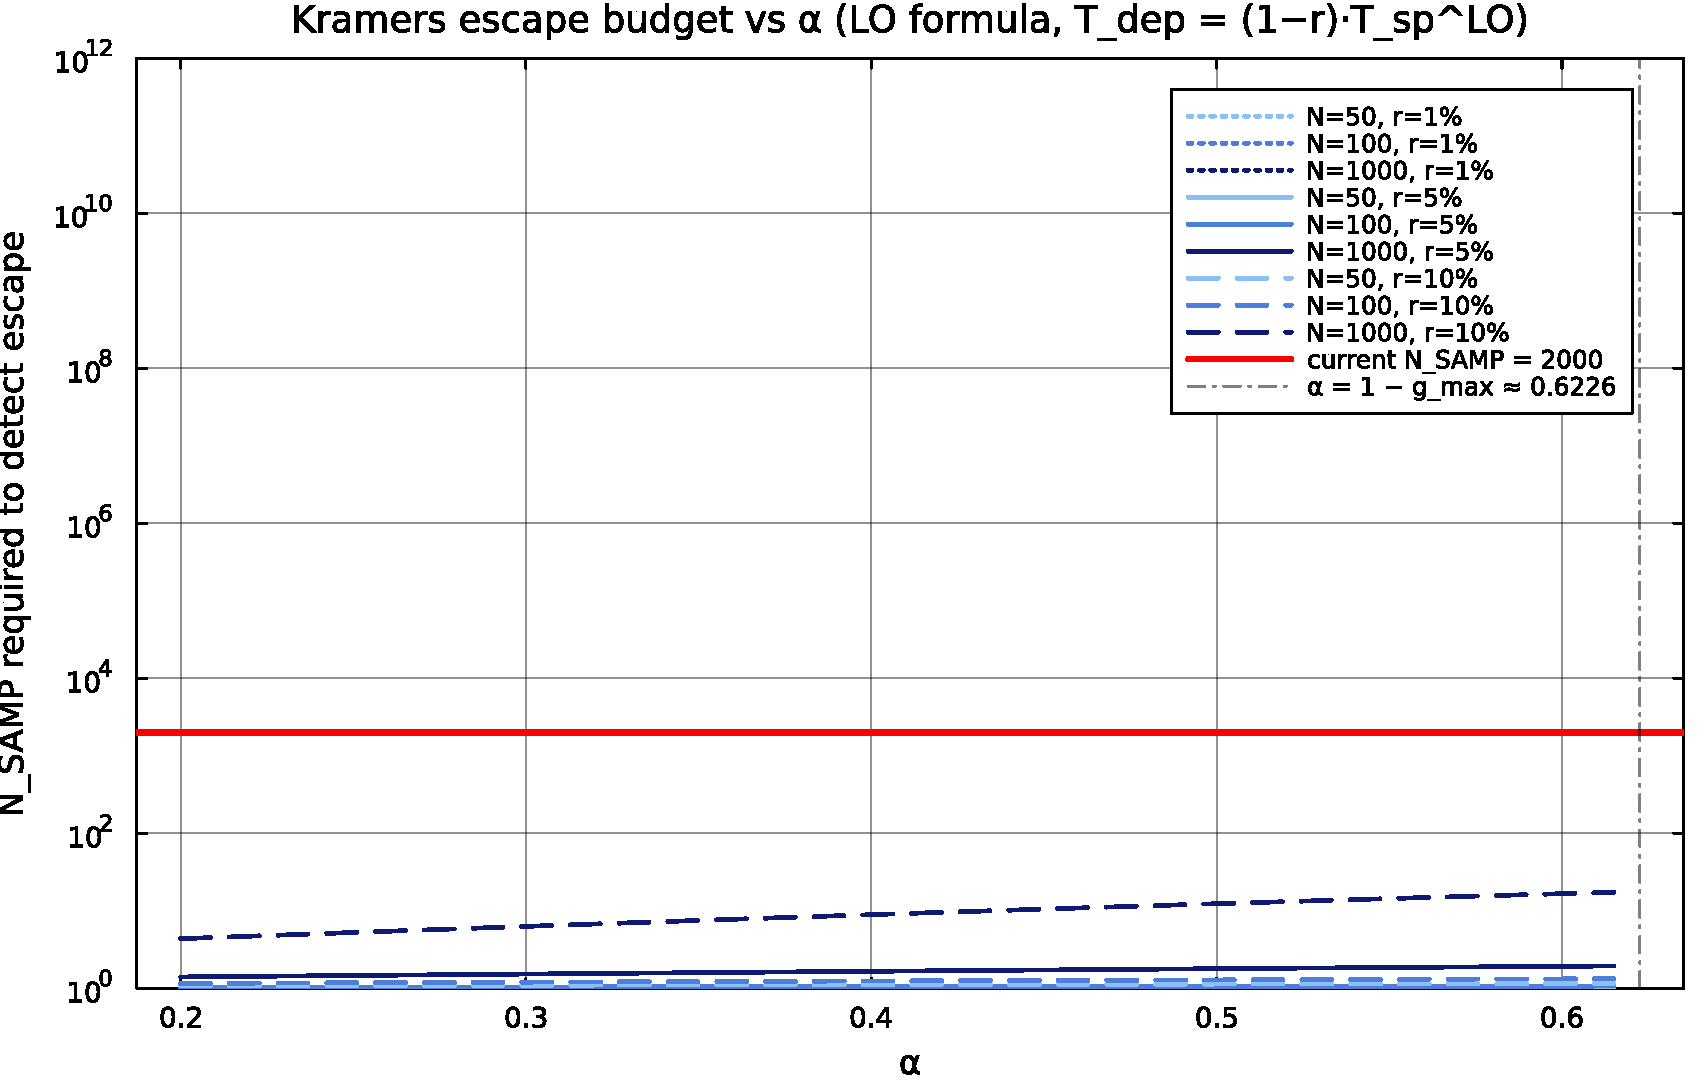
\includegraphics[width=0.85\linewidth]{panels_paper/budget_NSAMP_vs_alpha.pdf}
\caption{Kramers escape budget \eqref{eq:nsamp-req} versus $\alpha$
for $N \in \{50, 100, 1000\}$ at relative offsets $r \in \{1, 5,
10\}\%$ from $\Tsp^{\mathrm{LO}}(\alpha)$.  Red line: current MC
budget $N_{\mathrm{SAMP}} = 2{,}000$.  All curves sit far below the
red line, so the budget is sufficient at every $(\alpha, N)$ in the
window.  Dash-dot: cusp $\alpha = 1 - g_{\max} \approx 0.6226$.}
\label{fig:budget}
\end{figure}

\paragraph{Summary: which formula in which $\alpha$ interval.}
The thermodynamic boundary $\alpha_c(T)$ and the spinodal
$\Tsp(\alpha)$ are piecewise across the $\alpha$ axis.  Two
thresholds split the axis: $\alpha_{\mathrm{split}} \approx 0.241$
\eqref{eq:alpha-split}, where the interior saddle $\varphi^{*}$
enters the support, and $\alpha_{\mathrm{var}} \approx 0.336$
\eqref{eq:lvar-num}, where $S_{\mathrm{spur}}$ begins to
self-average.  In the master formula $\alpha_c(T) = 1 - g_{\max} -
\fret(T)$, the operative value of $g_{\max}$ depends on the
$\alpha$ range:

\begin{itemize}
\item \textbf{$\alpha < \alpha_{\mathrm{split}} \approx 0.241$}
(boundary regime).  The interior saddle of
$g(\varphi) = \tfrac12 \ln(1 - \varphi^2) + \Bnet\varphi$ lies
outside the natural integration range $[0, \varphi_{\max}(\alpha)]$;
the integrand is monotone and dominated by the support edge
$\varphi_{\max}(\alpha) = \sqrt{1 - \e^{-2\alpha}}$.  The correct
boundary is $\acBd(T)$ \eqref{eq:acbd}.  Self-averaging fails
here ($\alpha < \alpha_{\mathrm{var}}$), so even $\acBd(T)$ is only
a typical-value statement, not a sharp transition.  The Gaussian
formula $\acGauss(T)$ \eqref{eq:acgauss} agrees with $\acBd$ to
leading order in $\alpha$ but uses an inflated support edge
$\sqrt{2\alpha}$ instead of $\varphi_{\max}(\alpha)$.

\item \textbf{$\alpha_{\mathrm{split}} \leq \alpha < \alpha_{\mathrm{var}}
\approx 0.336$} (saddle-dominated mean, non-self-averaging).  The
interior saddle at $\varphi^{*} = (\sqrt 5 - 1)/2$ lies inside the
support and the saddle formula $\acSd(T)$ \eqref{eq:acsd} gives the
correct \emph{mean} boundary.  Sample-to-sample fluctuations in
$S_{\mathrm{spur}}$ are still exponentially large, so the boundary
position fluctuates from one disorder realization to the next; only
its mean is set by $\acSd$.

\item \textbf{$\alpha \geq \alpha_{\mathrm{var}} \approx 0.336$}
(saddle-dominated, self-averaging).  $\acSd(T)$ is the correct
boundary and the realization-to-realization spread vanishes
exponentially with $N$.  This is the regime where
\eqref{eq:acsd} should match Monte Carlo without finite-$N$ scatter
in $\alpha$.
\end{itemize}

\paragraph{Spinodal piecewise structure.}
The single-pattern spinodal $\acSp(T) = \phieq(T) - g_{\max}$
\eqref{eq:acsp} uses the same $g_{\max}$ as $\acSd$, so it carries
the same regime structure.  In the saddle regime
($\alpha > \alpha_{\mathrm{split}}$) it sits above $\acSd$ at
$T > 0$ and they meet at the endpoint
$(1 - g_{\max},\,0) \approx (0.6226,\,0)$.  Below
$\alpha_{\mathrm{split}}$ the LO derivation of $\acSp$ uses an
incorrect cusp position and \eqref{eq:acsp} does not apply; whether
a single-pattern spinodal exists in the boundary regime is a
separate question we do not address.  Within the saddle regime, the
LO formula \eqref{eq:acsp} is accurate at fixed $\alpha$ as long
as the basin offset $\xi$ exceeds the cusp-rounding window
\eqref{eq:rounding-window}, i.e.\ for $T$ not too close to
$\Tsp^{\mathrm{LO}}$ and for $\alpha$ not too close to the cusp
$1 - g_{\max}$.

% =========================================================================
\section{Monte Carlo methods}
\label{sec:mc}

All chains run on the $\sqrt{N}$-sphere with $\Bnet = 1$, Metropolis
updates, step size $\sigma(T) = 2.4\,T / \sqrt{N}$.  Three variants
differ in how they handle the $M = \e^{\alpha N}$ patterns.

\paragraph{Direct (all patterns).}
All $M$ patterns are generated and stored explicitly.  The chain
evaluates~\eqref{eq:lse} over all of them at every step.  Memory cost
is $O(N M)$; at $\alpha = 0.7$ and $N = 25$ this is
$M \approx 4 \times 10^7$ patterns, near the limit of a single GPU
with $40$~GB.  We use direct MC for the heatmap reference at $N = 25$
across $\alpha \in [0.20, 0.70]$.  Direct MC is impossible at the $N
\in \{50, 100, 1000\}$ used for the spinodal probe: $\e^{0.6 \cdot
1000} \approx 10^{260}$.

\paragraph{Semismart (saddle-band, anchored at $\bxi^1$).}
Only patterns with overlap $\varphi_{1\mu} \geq \varphi_{\mathrm{keep}}$
to the target $\bxi^1$ are stored explicitly.  $\varphi_{\mathrm{keep}}$
is chosen so that the expected number above the cutoff equals a budget
$K_{\mathrm{target}}$ (we use $K_{\mathrm{target}} = 10^4$); the actual
count $K_{\mathrm{kept}}$ is drawn from $\mathrm{Poisson}(M \cdot p)$
with $p = \Pr(\varphi > \varphi_{\mathrm{keep}})$, and the
$K_{\mathrm{kept}}$ overlap values are drawn from a truncated Beta
distribution.  The contribution of the discarded tail is the analytic
constant
\begin{equation}
\log C_{\mathrm{bulk}}
   = \alpha N + \ln\!\int_{-1}^{\varphi_{\mathrm{keep}}}
        f(\varphi)\,\e^{\Bnet N \varphi}\,\dd\varphi,
\label{eq:Cbulk}
\end{equation}
added inside the LSE log-sum at every step.

The retained set is quenched: each disorder sample fixes the retained
patterns once and reuses them for the chain.  At cold init the chain
stays near $\bxi^1$, so the kept patterns dominate the local energetics
of escape; the bulk acts as a smooth background.

\paragraph{Smart (top-K, dynamic anchor).}
Same as semismart, but the retained set is refreshed every
$N_{\mathrm{REFRESH}}$ steps based on the chain's current position.
Used in the LSE Nramp scripts where the chain wanders far from
$\bxi^1$.  The spinodal probe is a cold-init experiment with negligible
chain wandering, so we use semismart, not smart.

\paragraph{What each variant measures.}
Direct MC measures the true thermodynamics at fixed $N$.  Semismart MC
faithfully measures the local stability of the retrieval well around
$\bxi^1$ (the spinodal) and reproduces the saddle thermodynamics through
$C_{\mathrm{bulk}}$.  Smart MC tracks the chain across the energy
landscape and is needed when the chain leaves the single-pattern basin
and explores the saddle phase.

\paragraph{Top-K vs.\ saddle patterns.}
Two pattern populations matter in LSE thermodynamics.  Patterns with
high $\varphi_{1\mu}$ (top-K) are the strongest competitors at the
retrieval well: they set the local curvature of $H$ at $\bx = \bxi^1$
and therefore the spinodal.  The saddle constellation patterns at
$\varphi \approx 0.618$ have random (typically near-zero) overlap with
$\bxi^1$.  They do not enter the local stability of the retrieval well;
they enter $\acSd$ through the partition-function competition with
$\fret(T)$.  Semismart MC samples top-K and is the right tool for the
spinodal.  The saddle thermodynamics is added analytically through
$C_{\mathrm{bulk}}$, not measured by the chain.

% =========================================================================
\section{What we have}
\label{sec:result}

Two datasets so far:
\begin{enumerate}
\item Heatmap at $N = 25$, $\alpha \in [0.20, 0.70]$ step $0.01$,
$T \in [0.025, 0.500]$ on $40$ points, using direct MC and semismart MC
on the same grid.  Cell value: $\avg{\phi} - \phieq(T)$ averaged over
disorder.  See \Cref{fig:heatmap}.
\item Spinodal probe: semismart MC at
$\alpha \in \{0.20, 0.25, \ldots, 0.60\}$, $N \in \{50, 100, 1000\}$,
cold init only, per-$\alpha$ fine $T$ grids, $8$ disorders, ceiling at
$T = 0.5$ (cells with $\avg{\phi}/\phieq > 0.9$ at $T = 0.5$ are
reported as NaN).  See \Cref{tab:anchors}.
\end{enumerate}

\begin{figure}[t]
\centering
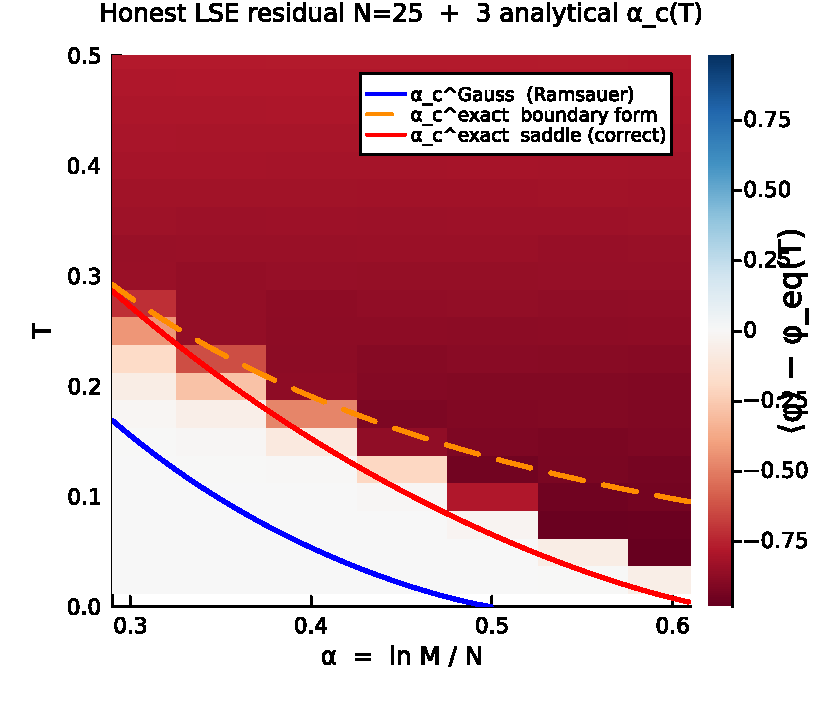
\includegraphics[width=0.95\linewidth]{panels_paper/heatmap_LSE_AAAI_residual_3boundaries.pdf}
\caption{Residual $\avg{\phi} - \phieq(T)$ from direct and semismart
MC at $N = 25$, with the three boundary curves \eqref{eq:acgauss},
\eqref{eq:acbd}, \eqref{eq:acsd} overlaid.  Filled circles: empirical
cold-init spinodal anchors $\Tsp^{\mathrm{MC}}(\alpha, N)$ at
$N \in \{50, 100, 1000\}$ (light to dark blue).  Violet dashed line:
leading-order spinodal $\acSp(T)$ from \eqref{eq:acsp}.}
\label{fig:heatmap}
\end{figure}

\paragraph{Heatmap.}
\Cref{fig:heatmap} shows three things.  First, the Gaussian curve
$\acGauss$ sits deep inside the spin-glass region for the whole
range.  Second, the boundary transplant $\acBd$ sits far outside the
empirical transition.  Third, the saddle curve $\acSd$ tracks the
empirical transition for $\alpha \gtrsim 0.45$ at $N = 25$.  At
$\alpha < 0.45$ the empirical transition lies at lower $T$ than $\acSd$
predicts.

\paragraph{Spinodal anchors.}
\Cref{tab:anchors} reports the cold-init boundary $\Tsp^{\mathrm{MC}}$
detected as the temperature at which $\avg{\phi}$ first drops below
$0.9\,\phieq(T)$.  The leading-order prediction \eqref{eq:acsp} is
shown for comparison.

\begin{table}[h]
\centering
\caption{Empirical spinodal $\Tsp^{\mathrm{MC}}$ from cold-init semismart
MC, compared to leading-order $\Tsp^{\mathrm{LO}}$ from \eqref{eq:acsp}.
$\mathrm{NaN}$ means no departure detected by the ceiling $T = 0.5$.}
\label{tab:anchors}
\begin{tabular}{c|ccc|c}
\hline
$\alpha$ & $N=50$ & $N=100$ & $N=1000$ & $\Tsp^{\mathrm{LO}}$ \\
\hline
$0.20$ & $0.481$ & NaN     & NaN     & $1.154$ \\
$0.25$ & $0.426$ & NaN     & NaN     & $0.966$ \\
$0.30$ & $0.384$ & $0.455$ & NaN     & $0.799$ \\
$0.35$ & $0.322$ & $0.365$ & NaN     & $0.647$ \\
$0.40$ & $0.272$ & $0.298$ & $0.454$ & $0.509$ \\
$0.45$ & $0.194$ & $0.218$ & $0.347$ & $0.381$ \\
$0.50$ & $0.122$ & $0.154$ & $0.244$ & $0.262$ \\
$0.55$ & $0.071$ & $0.082$ & $0.150$ & $0.151$ \\
$0.60$ & $0.028$ & $0.029$ & $0.081$ & $0.046$ \\
\hline
\end{tabular}
\end{table}

Three observations.

(1) For fixed $\alpha$, $\Tsp^{\mathrm{MC}}(\alpha, N)$ increases
monotonically with $N$ toward $\Tsp^{\mathrm{LO}}(\alpha)$.  At
$\alpha = 0.55$, $N = 1000$ the empirical and LO values agree.

(2) For $\alpha \in [0.30, 0.50]$, $\Tsp^{\mathrm{MC}}(\alpha, 1000)$
sits below $\Tsp^{\mathrm{LO}}(\alpha)$.  This is the expected sign of
subleading $1/N$ corrections to the spinodal.

(3) At $\alpha = 0.60$, $N = 1000$, $\Tsp^{\mathrm{MC}} = 0.081$ sits
\emph{above} $\Tsp^{\mathrm{LO}} = 0.046$.  The budget analysis
(\Cref{fig:budget}, \cref{sec:spinodal-budget}) rules out a
finite-MC-time floor: the LO Kramers shift at this cell is at most
$0.008$, four times smaller than the observed gap.  The deviation is
an NLO correction to the spinodal location itself.  In this regime
$\xi \lesssim \log N / N$ at $T = \Tsp^{\mathrm{LO}}$, so the
parabolic LO barrier vanishes and the cusp-rounded NLO physics
dominates.

\paragraph{Hot init not yet run.}
The hot-init column $\Tsp^{\mathrm{hot}}$ in
\texttt{spinodal\_summary.csv} is uniformly NaN: the run used
cold init only.  The hot-init boundary identifies the thermodynamic
$T_c^{\mathrm{sd},\mathrm{MC}}(\alpha)$ and, paired with cold init,
delimits the metastability band.  This is the most important missing
piece.

% =========================================================================
\section{What is left}
\label{sec:left}

The status of each task: \emph{done}, \emph{in progress}, \emph{open}.

\paragraph{Numerical tasks.}

\begin{description}
\item[1. Hot-init spinodal probe] (\emph{open}).
Add hot init (uniform sphere start) at the same
$(\alpha, N, T)$ grid as the cold-init run.  Cold and hot boundaries
together delimit the metastability band; cold $\to \acSp$,
hot $\to \acSd$.

\item[2. Finite-MC-time test at $\alpha = 0.60$, $N = 1000$]
(\emph{closed by analysis}).
Settled by \Cref{fig:budget}: LO Kramers shift at this cell is
$\le 0.008$, far below the observed $0.035$ gap.  The deviation is
NLO, not finite-MC-time.  An MC re-run with larger
$N_{\mathrm{SAMP}}$ would not move the empirical $\Tsp^{\mathrm{MC}}$.

\item[3. Extension of spinodal anchors toward the cusp]
(\emph{open}).
Add $\alpha \in \{0.605, 0.610, 0.615, 0.620, 0.625\}$ with
extended $N_{\mathrm{SAMP}}$.  Goal: confirm that the empirical curve
bends to $T = 0$ at $\alpha = 1 - g_{\max} \approx 0.6226$.

\item[4. Smart-MC heatmap at larger $N$]
(\emph{open}).
The heatmap is at $N = 25$.  The saddle-band-keeping semismart code
runs at $N \in \{50, 100, 1000\}$.  An $N = 50$ heatmap over
$\alpha \in [0.20, 0.70]$ on the same $T$ grid would show whether the
discrepancy at $\alpha < 0.45$ at $N = 25$ shrinks with $N$
(thermodynamic correction) or persists (kinetic effect).

\item[5. Chain-length scan]
(\emph{open}).
Fix $(\alpha, T)$ inside the small-$\alpha$ discrepancy
region.  Sweep $N_{\mathrm{chain}}$ over factor-of-four steps from
$2^{14}$ to $2^{22}$.  Drift of the residual toward $\acSd$ as
$\log N_{\mathrm{chain}}$ grows = kinetic escape.  Flat residual =
thermodynamic finite-$N$ correction.

\item[6. Direct measurement of the Kramers barrier]
(\emph{open}).
Long chain inside the basin gives the histogram
$P(\varphi_1)$ and hence $V_{\mathrm{eff}}(\varphi_1) = -T \ln
P(\varphi_1)$.  Read $\Delta F$ from the histogram and predict the
escape time by Arrhenius.

\end{description}

\paragraph{Analytical tasks.}

\begin{description}

\item[7. Subleading $1/N$ corrections to $\acSp$]
(\emph{open}).
Expand \eqref{eq:F-leading} beyond leading order.  Two
sources, both discussed in \Cref{sec:spinodal}: cusp rounding at
scale $1/(\Bnet N)$ in $\varphi_1$, and the extreme-value
correction below the self-averaging threshold $\alpha_{\mathrm{var}}
\approx 0.336$.  Goal: quantitative prediction of
$\Tsp(\alpha, N)$ to compare against the empirical anchors at
$N \in \{50, 100, 1000\}$.

\item[8. Spinodal formula from the exact-density free energy]
(\emph{open}).
Re-derive \eqref{eq:acsp} from the same exact-density partition
function that yields $\acSd$, without the leading-order
saddle approximation.  Goal: close the gap between the empirical
$\Tsp^{\mathrm{MC}}$ at $\alpha = 0.30$, $N = 1000$ (NaN — no
departure detected) and the LO value $\Tsp^{\mathrm{LO}} = 0.80$.

\item[9. LSE Kramers barrier]
(\emph{open}).
Derive $\Delta F(\alpha, T)$ for escape from the LSE
retrieval well in closed form.  The LSE landscape is smooth (no LSR
support cutoff), so the escape mechanism differs from the LSR centroid
hopping of~\citep{petrova2026metastable}.  Goal: analytic Arrhenius
form to compare with task 6.

\end{description}

\paragraph{Writing tasks.}

\begin{description}

\item[10. Figure of the empirical anchors vs.\ LO]
(\emph{done}: included in \Cref{fig:heatmap}).

\item[11. Caption pass]
(\emph{open}).  Figures and tables to be rewritten to match
the report style.

\item[12. References]
(\emph{open}).  \texttt{refs.bib} contains the four citations
used here; check that all keys resolve in the final PDF.

\end{description}

\paragraph{Decision points for the user.}
Two choices shape the next sprint.  First: do we treat the
small-$\alpha$ discrepancy as kinetic or thermodynamic?  Tasks 4--6
discriminate.  Second: does the paper claim
$\acSd(0) = 1 - g_{\max} \approx 0.6226$ as the corrected Ramsauer
threshold, or does it remain in the present descriptive form
(``saddle dominates; transplant is wrong; here is the curve'')?
The first claim is stronger and would benefit from task 4 first.

% =========================================================================
\bibliographystyle{plain}
\bibliography{refs}

\end{document}
